\section{Обходы графа II}
\subsection{Условие задания}
\textbf{Вариант 27:} Найти длины кратчайших (по числу дуг) путей из вершины $u$ во все остальные.

\subsection{Примеры исходного кода}
Для нахождения длины кратчайших путей из вершины $u$ во все остальные
был объявлен метод \mitext{shortestPathLengthsFrom()}, принимающий
метку вершины $u$ и возвращающий расстояния до всех вершин графа (по числу дуг):
\begin{minted}{typescript}
shortestPathLengthsFrom(u: string): Map<string, number> {
  if (!this.adj.has(u)) {
    throw new NodeNotExists(u)
  }

  const shortestPaths: Map<string, number> = new Map()

  for (const node of this.adj.keys()) {
    shortestPaths.set(node, Infinity) // пока считаем, что расстояния до других узлов бесконечность
  }
  shortestPaths.set(u, 0) // расстояние до самого себя 0

  const queue = [u] // очередь обхода
  while (queue.length > 0) {
    const currentNode = queue.shift()!
    const neighbors = this.adj.get(currentNode)!

    for (const neighbor of neighbors.keys()) {
      if (shortestPaths.get(neighbor) === Infinity) { // если узел еще не был посещен
        // установить кратчайшее расстояние до него
        shortestPaths.set(neighbor, shortestPaths.get(currentNode)! + 1)
        queue.push(neighbor) // добавить соседний узел в очередь обхода
      }
    }
  }

  return shortestPaths
}
\end{minted}

\subsection{Краткое описание алгоритма}
Этот алгоритм использует метод обхода в ширину (BFS) для нахождения кратчайших путей.

Создается \mitext{Map<string, number>}, где для каждой вершины устанавливается начальное расстояние.
Расстояние от $u$ до самой себя равно $0$, а до остальных вершин "--- бесконечность.

Используется очередь для обхода графа. Начальная вершина $u$ добавляется в очередь.
Пока очередь не пуста, извлекается текущая вершина. Для каждого соседнего узла проверяется,
был ли он уже посещен. Если не был, устанавливается кратчайшее расстояние и добавляется в очередь.

\subsection{Примеры входных и выходных данных}
\subsubsection{Входные данные}
\begin{figure}[H]
  \begin{minipage}{0.5\textwidth}
    \centering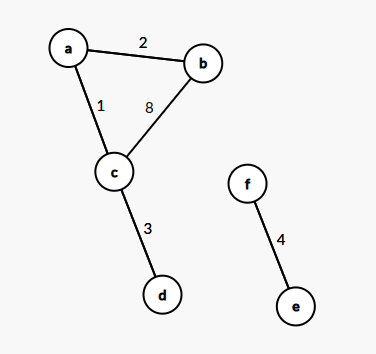
\includegraphics[width=0.6\linewidth]{figs/task-6/graph-6.png}
  \end{minipage}
  \begin{minipage}{0.5\textwidth}
    \centering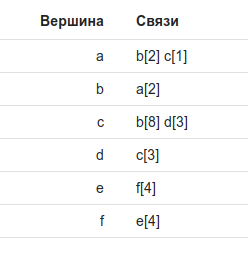
\includegraphics[width=0.6\linewidth]{figs/task-6/adj-6.png}
  \end{minipage}
  \caption{Неориентированный граф}
\end{figure}

\begin{minted}{js}
{
  "weighted": true,
  "oriented": false,
  "adj": {
    "a": {
      "b": 2,
      "c": 1
    },
    "b": {
      "a": 2
    },
    "c": {
      "a": 1,
      "d": 3
    },
    "d": {
      "c": 3
    },
    "e": {
      "f": 4
    },
    "f": {
      "e": 4
    }
  }
}
\end{minted}

\subsubsection{Выходные данные}
\begin{figure}[H]
  \centering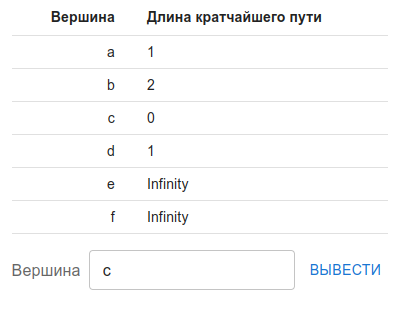
\includegraphics[width=0.4\textwidth]{figs/task-6/res-6.png}
  \caption{Результат работы}
\end{figure}